% Created 2019-11-25 Mon 20:35
% Intended LaTeX compiler: pdflatex
\documentclass[a4paper, justified, notitlepage, sfsidenotes, notoc]{tufte-book}
     \input{/users/rakhim/.emacs.d/latex/tufte.tex}
\usepackage[utf8]{inputenc}
\usepackage[T1]{fontenc}
\usepackage{graphicx}
\usepackage{grffile}
\usepackage{longtable}
\usepackage{wrapfig}
\usepackage{rotating}
\usepackage[normalem]{ulem}
\usepackage{amsmath}
\usepackage{textcomp}
\usepackage{amssymb}
\usepackage{capt-of}
\usepackage{hyperref}
\date{}
\title{Computer Science For The Busy Developer}
\hypersetup{
 pdfauthor={Rakhim Davletkaliyev},
 pdftitle={Computer Science For The Busy Developer},
 pdfkeywords={},
 pdfsubject={},
 pdfcreator={Emacs 26.3 (Org mode 9.1.9)},
 pdflang={English}}
\begin{document}

\part{Subset, superset}
\label{sec:org25368f9}

When all members of set \(A\) are present in another set \(B\), then \(A\) is a \textbf{subset} of \(B\). Let's say set \(B\) is the set of all movies ever produced. Then \(A\) (movies I've watched) is clearly a subset of \(B\). This notion is expressed like so:

\begin{equation}
A \subseteq B
\end{equation}

To look at things from the other end, \(B\) is a \textbf{superset} of \(A\):

\begin{equation}
B \supseteq A
\end{equation}

\begin{marginfigure}
  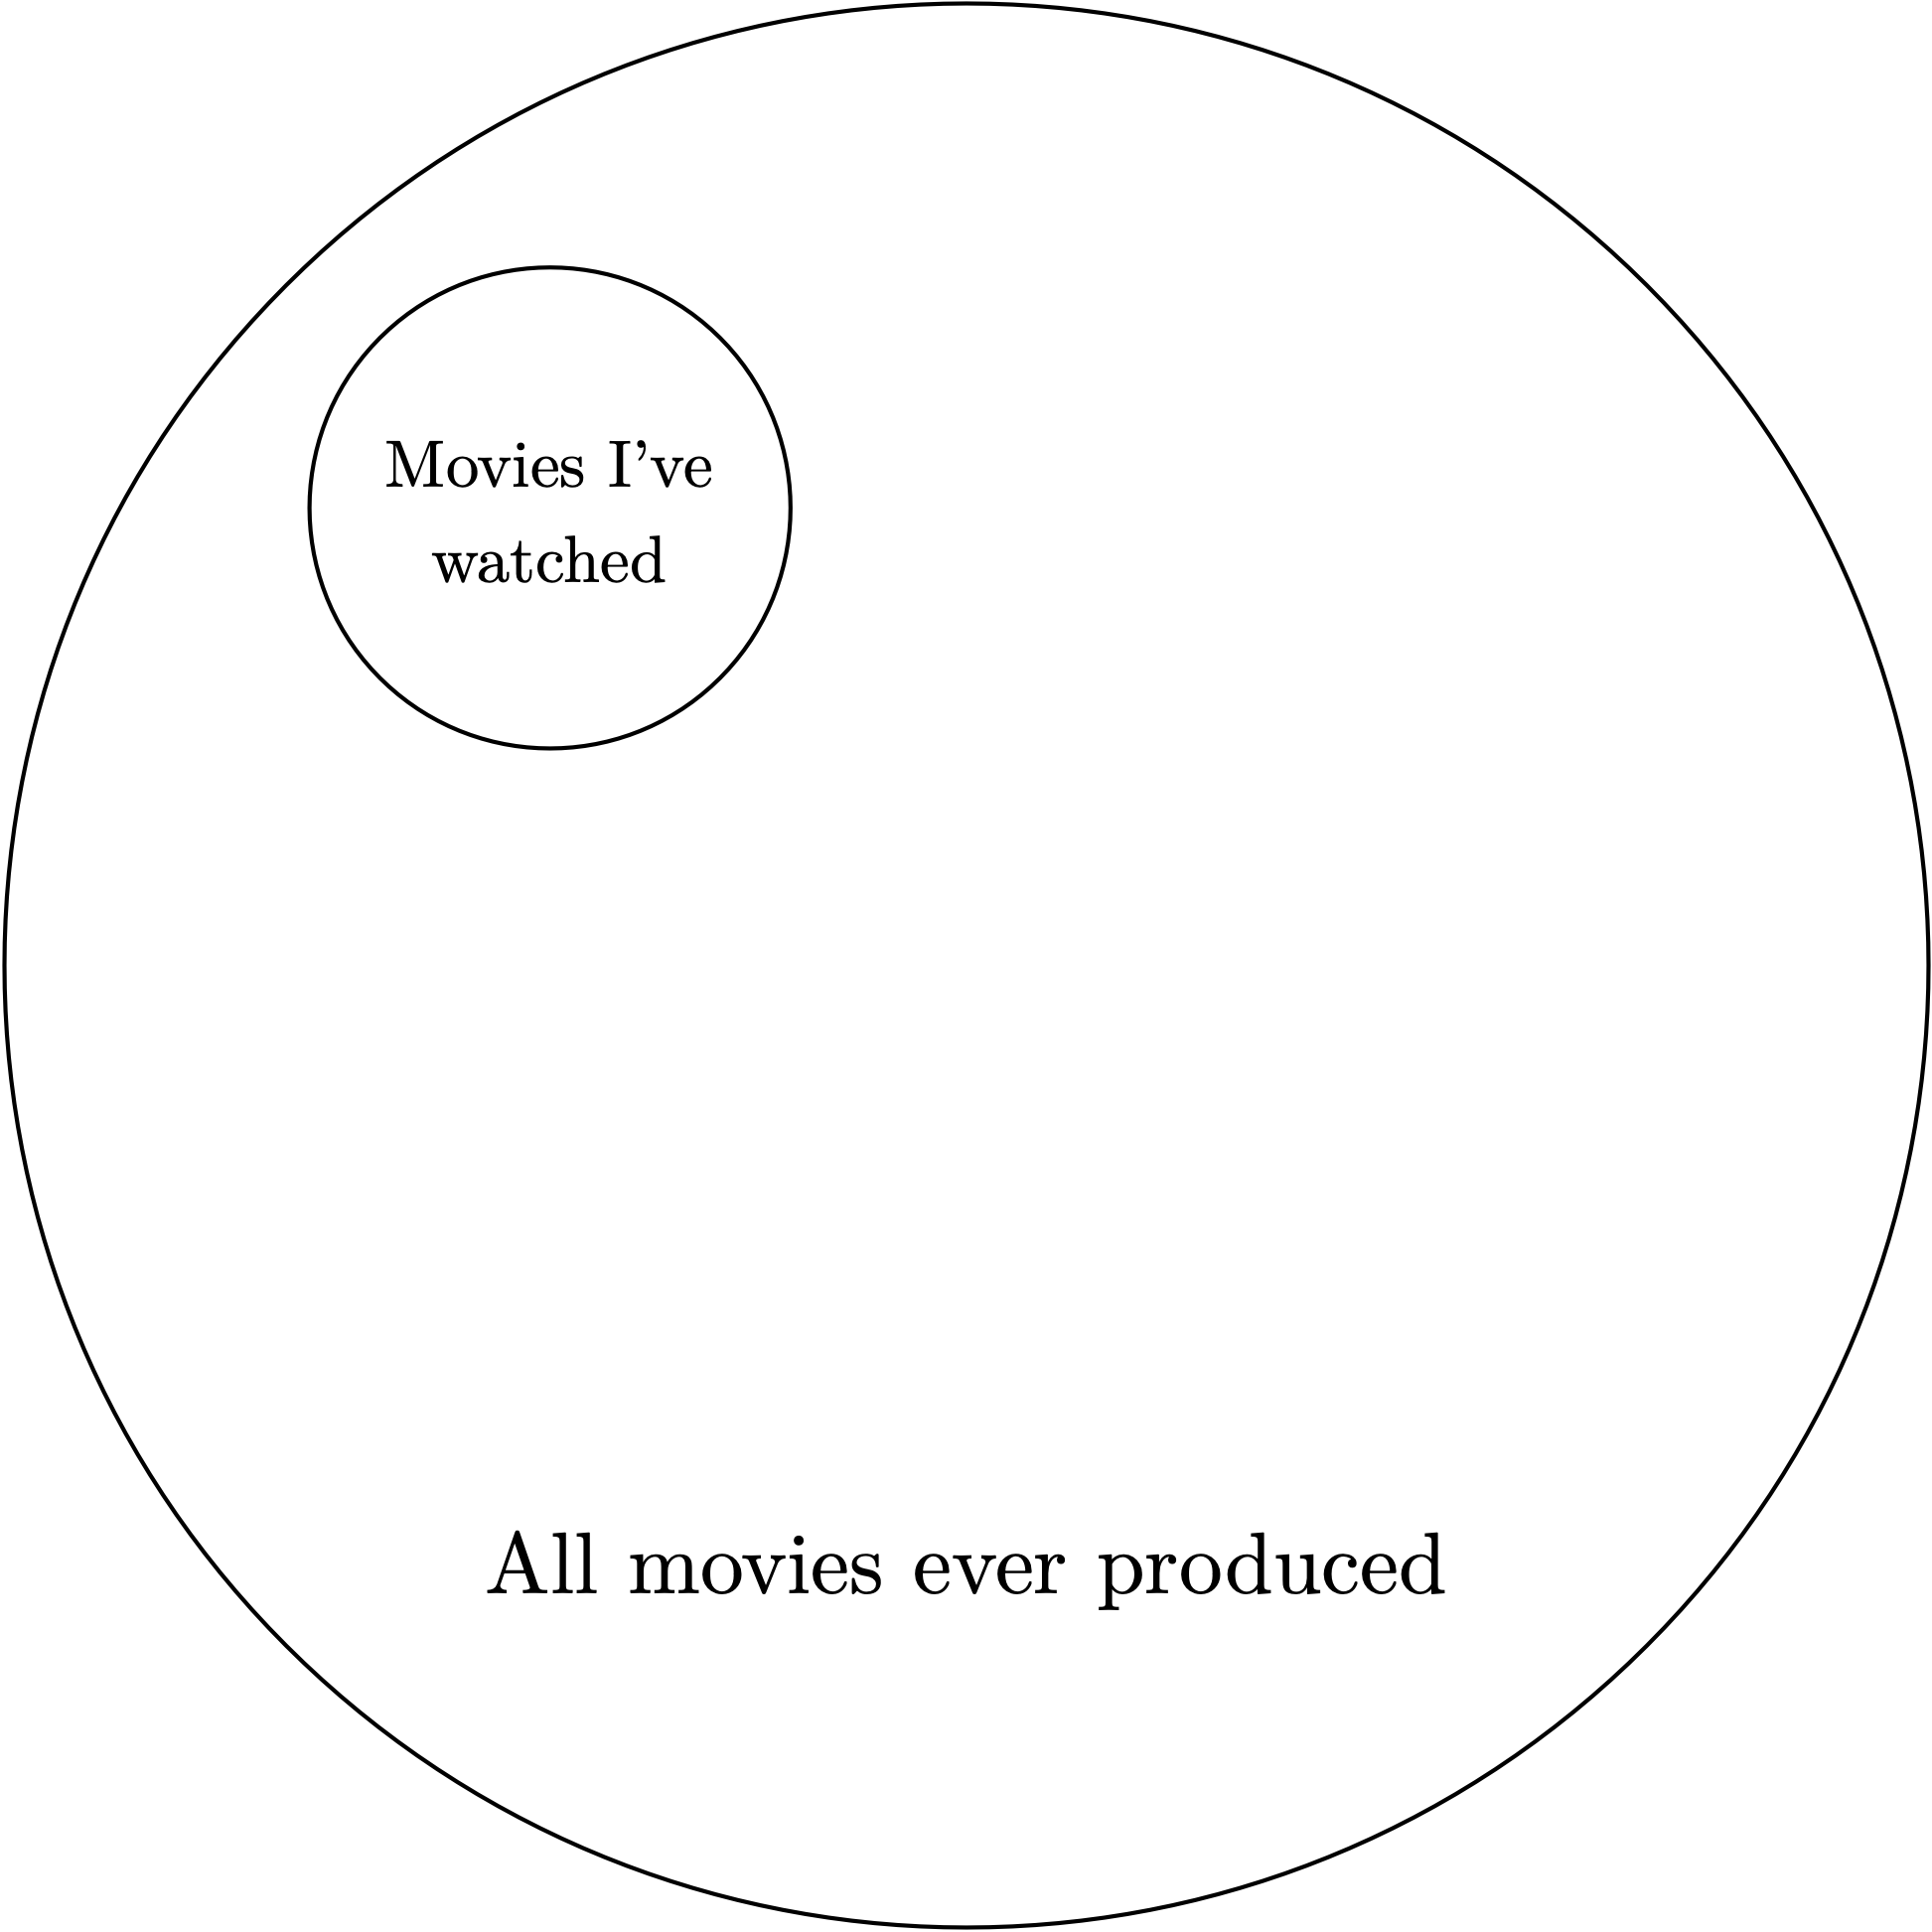
\includegraphics[width=\linewidth]{images/subset.png}
  \caption{A set and its subset.}
  \label{fig:marginfig}
\end{marginfigure}


You know what else is a subset of \(B\)? An empty set!

\begin{equation}
\varnothing \subseteq B
\end{equation}

This either sounds absolutely natural to you or extremely weird. It makes perfect sense to a mathematician, because it's easy to argue: \emph{all} members of \(\varnothing\) are present in \(B\), all zero of them.

It gets weirder. As per our definition, if all members of a set are also present in another set, then the one is a subset of the other. This means any set is a subset of itself.

\begin{equation}
A \subseteq A \\
B \subseteq B \\
Z \subseteq Z
\end{equation}

By extension, if two sets are the same, then either of them is a subset of the other.

\begin{equation}
\textrm{if } A \subseteq B \textrm{ and } B \subseteq A \textrm{ then } A = B
\end{equation}

---

When we look at a statement \(A \subseteq B\), we often need to know whether \(A = B\) or not. To distinguish between the two cases, mathematicians use a special notion of a \textbf{proper subset}.

If \(A \in B\), but \(A \neq B\), then \(A\) is a proper subset of \(B\).

\begin{equation}
A \subset B
\end{equation}

Since I haven't watched all the movies ever produced, I can say that \(A\) is a proper subset of \(B\). So, a set is a subset of itself, but is never a proper subset of itself.
\end{document}
